% \newpage
% \begin{center}
% \normalfont\Large\bfseries MPC exercise: week four
% \end{center}
\setcounter{section}{0}
\setcounter{figure}{0}
\section{Pre-set}

\begin{enumerate}
    \item Consider the system 
\begin{align*}
    x_{k+1} &=\begin{bmatrix}
        0&1\\
        -1&0
    \end{bmatrix}x_k.\\
\end{align*}
If $x\in \mathcal{X}$, $\mathcal{X} =\{x| \begin{bmatrix}
        1&1\\
        -1&-1\\
        1&0\\
        -1&0
    \end{bmatrix}x\leq\begin{bmatrix}
        1\\
        1\\
        1\\
        1
    \end{bmatrix}\}$,
    sketch the set $\mathcal{X}$ and pre-set of $\mathcal{X}$. Compute the successor state of a few points in $\text{pre($\mathcal{X}$)}$ to convince yourself it is correct.

    \solution{See the Fig. \ref{ex4}
    \begin{figure}[htbp]
        \centering
        \begin{minipage}{0.35\textwidth}
            \centering
            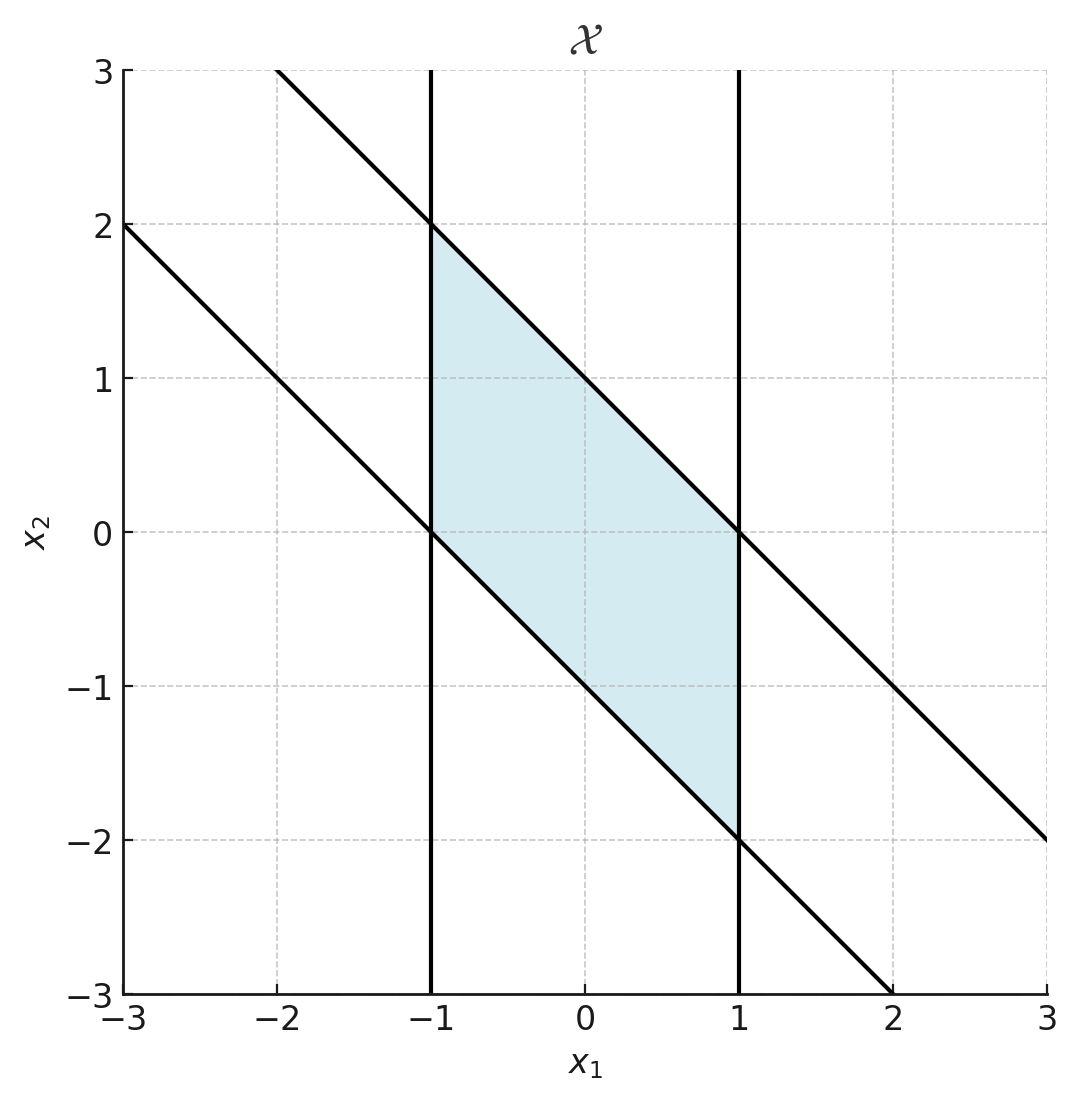
\includegraphics[width=\linewidth]{fig/original set.png}
            \caption*{Original set.}
        \end{minipage}\hspace{25pt}
        \begin{minipage}{0.35\textwidth}
            \centering
            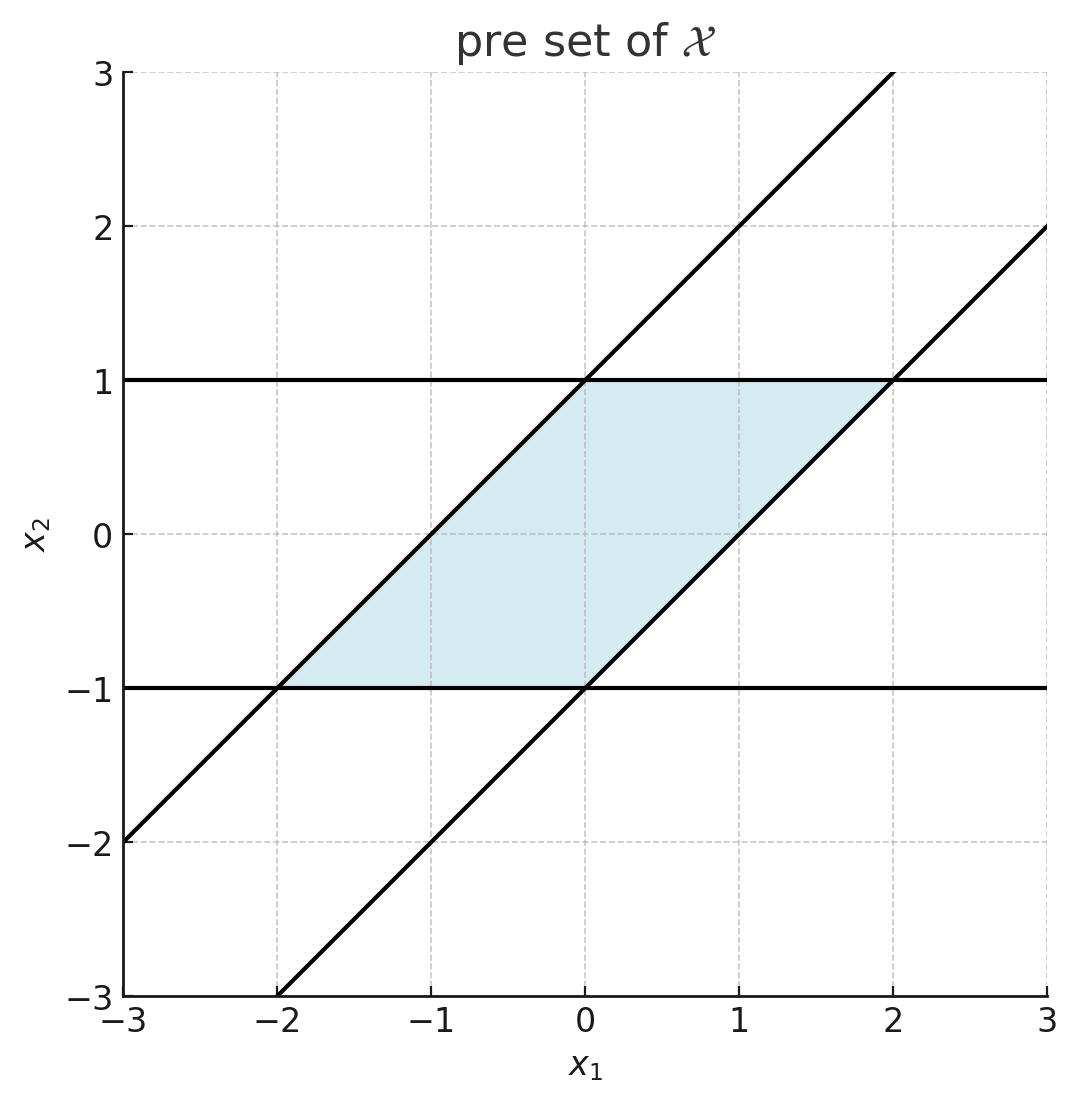
\includegraphics[width=\linewidth]{fig/pre set.png}
            \caption*{Pre set.}
        \end{minipage}
        \caption{Solution of problem 1.1.}
        \label{ex4}
    \end{figure}}
    
    \item Consider the system $x_{k+1} = 0.5x_k + u_k$. Calculate and plot the pre-set if $x\in [-2, 2]$ and $u\in [-1,1]$.

    \solution{For the pre set, we have 
    \begin{equation*}
        \begin{bmatrix}
            0.5&1\\
            -0.5&-1\\
            0&1\\
            0&-1
        \end{bmatrix}\begin{bmatrix}
            x_k\\
            u_k
        \end{bmatrix}\leq
        \begin{bmatrix}
            2\\
            2\\
            1\\
            1
        \end{bmatrix}.
    \end{equation*}
    \begin{figure}[htbp]
        \centering
        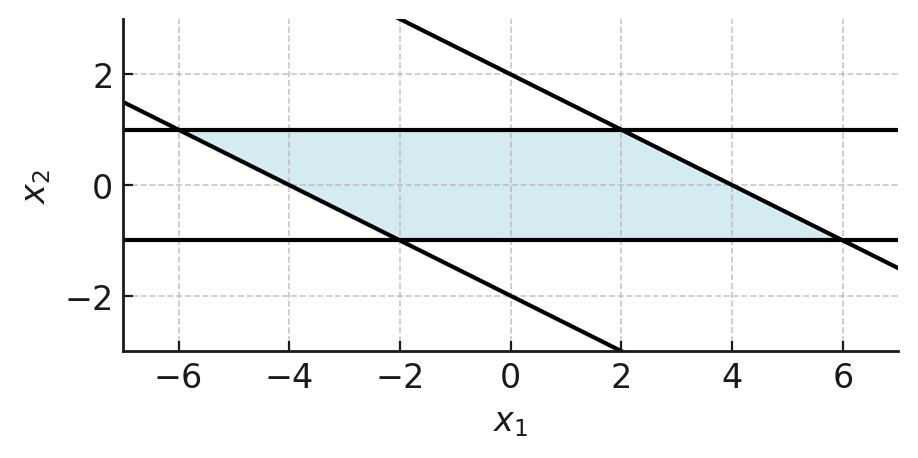
\includegraphics[width=0.5\linewidth]{fig/control pre set.png}
        \caption{Solution of problem 1.2.}
    \end{figure}
    Projecting the feasible set onto the $x$-axis, we conclude that the pre set for $x$ is $[-6,6]$.}\vspace{5\baselineskip}
\end{enumerate}


\section{Invariant set}
\begin{enumerate}
    \item Consider the system $x_{k+1} = \begin{bmatrix}
        0&1\\
        -1&0
    \end{bmatrix}x_k$ and the constraint $\{x|\begin{bmatrix}
        1&1\\
        -1&-1\\
        1&-1\\
        -1&1
    \end{bmatrix}x\leq\begin{bmatrix}
        1\\
        1\\
        1\\
        1
    \end{bmatrix}\}$. Calculate and plot the maximum invariant set. 
    
    \solution{See Fig. \ref{ex41}
    \begin{figure}[h]
        \centering
        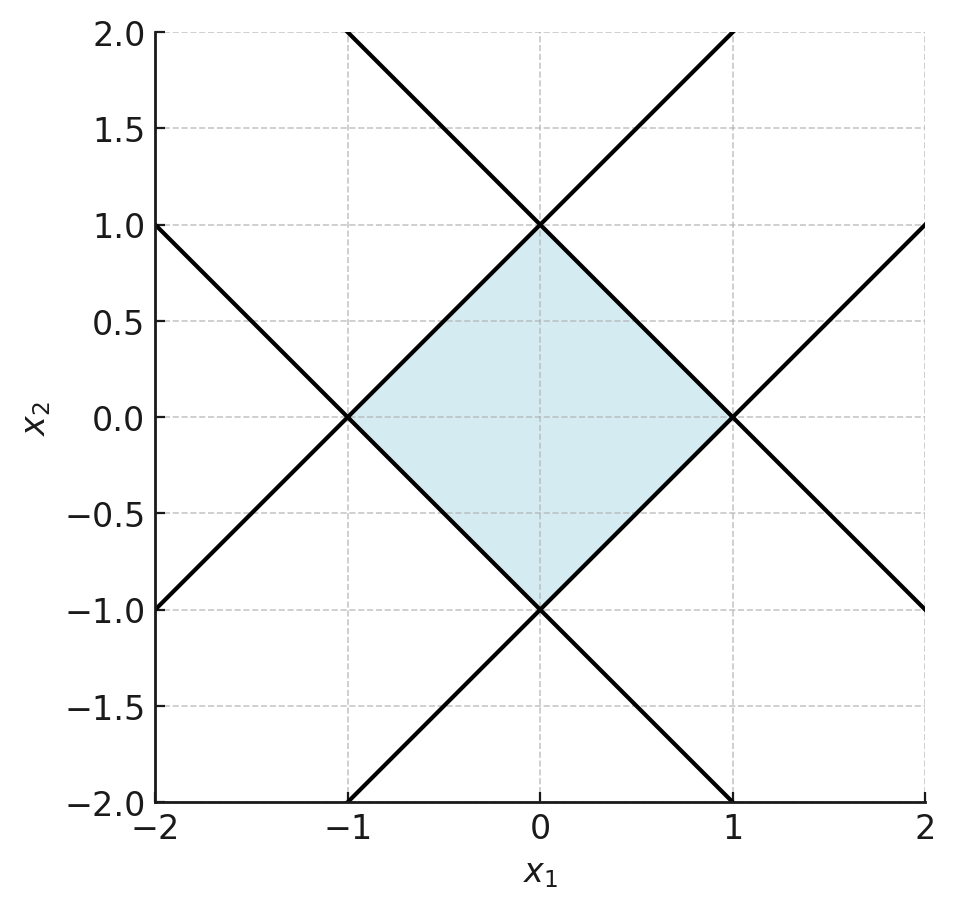
\includegraphics[width=0.5\linewidth]{fig/invariant set.png}
        \caption{Solution of problem 2.1.}
        \label{ex41}
    \end{figure}}
    
    \item Consider the nonlinear system $x_{k+1} = x_k^2 + u_k$, where $x\in [-2,2]$, $u\in [-1,1]$. Calculate the maximum control invariant set. (Hint: Consider a sequence, $a_{k+1} = \sqrt{a_k+1}$, if $a_0 \geq \frac{1+\sqrt{5}}{2}\approx 1.618$, then $a_{k+1}\leq a_k$, and $\lim_{k\rightarrow\infty}a_k = \frac{1+\sqrt{5}}{2}$)

    \solution{We perform the iteration for calculating the maximum control invariant set. Let $\Omega_i$ be the set sequence. $\Omega_0 = [-2,2]$. $\text{pre}(\Omega_0)$ is the set that $\exists u\in[-1,1]$ such that $x^2+u\in[-2,2]$. Hence $x^2\in[-3,3]$, $x\in[-\sqrt{3},\sqrt{3}]$. $\text{pre}(\Omega_0) = [-\sqrt{3},\sqrt{3}]$. $\Omega_1 = \Omega_0\cap\text{pre}(\Omega_0) = [-\sqrt{3},\sqrt{3}]$. $\text{pre}(\Omega_1) = [-\sqrt{\sqrt{3}+1},\sqrt{\sqrt{3}+1}]$. $\Omega_2 = \Omega_1\cap\text{pre}(\Omega_1) = [-\sqrt{\sqrt{3}+1},\sqrt{\sqrt{3}+1}]$. Hence $\Omega_{k+1} = [-a_k,a_k]$, where $a_{k+1} = \sqrt{a_k+1}, a_0 = \sqrt{3}\geq 1.618$. $\Omega_{\infty} = [-\frac{1+\sqrt{5}}{2},\frac{1+\sqrt{5}}{2}]$.}
    \item Given a system $x_{k+1} = f(x_k)$, which has a Lyapunov function $V$. (Recall a Lyapunov function has the property $V(f(x_k))\leq V(x_k)$). Prove that the set $\{x|V(x)\leq \alpha\}$ is invariant for all $\alpha\geq 0$.
    
    \solution{We need to prove that $\forall x_k \in \mathcal{X}$, where $ \mathcal{X}:= \{x
    |V(x)\leq \alpha\}$, $x_{k+1}\in \mathcal{X}$. If $x_k \in\mathcal{X}$, $V(x_k)\leq\alpha$. Since $V(x)$ is a Lyapunov function, $V(x_{k+1})\leq V(x_k)\leq \alpha$. Hence $x_{k+1}\in\mathcal{X}$.}
\end{enumerate}